\originalchapter{2017至2019年期末及练习卷}
本章保留各卷原题号与最细子问. 正式期末卷的解答均为依据官方解答重构, 补齐推导; 原解答的笔误在相应位置注明. Practice中只有外部阅读指引的题目另标为AI补写推导. 熵的对数以2为底, 正态分布函数记为 $\Phi$. 未注明时, 连续密度在所列支集外均为零. 各离散过程使用题中全部已观察历史生成的过滤.

\originalsection{2017年春季期末卷}
题卷与\href{https://ocw.mit.edu/courses/18-600-probability-and-random-variables-fall-2019/resources/mit18_600f19_final_2017/}{官方题目}, \href{https://ocw.mit.edu/courses/18-600-probability-and-random-variables-fall-2019/resources/mit18_600f19_final_2017_soln/}{官方解答}对应. 全卷100分, 原卷要求清楚展示计算且框出最终结果.

\begin{exercise}\label{ex:fl17-1}
原卷第1题(10分). $X\sim\Exp(1)$. (a) 求 $\E[3X^{13}]$. (b) 求 $\Prob(X>10\mid X>5)$. (c) 令 $Y=X^2$, 求分布函数 $F_Y$.
\end{exercise}
\begin{solution}
(a)\label{sol:fl17-1-a} 对非负整数 $m$, 分部积分给出
$\int_0^\infty x^m\ee^{-x}\dd x=m\int_0^\infty x^{m-1}\ee^{-x}\dd x$, 边界项为零. 从 $m=0$ 的积分1逐次递推, 得 $\E X^m=m!$. 因此答案为 $3\cdot13!$.
(b)\label{sol:fl17-1-b} 两事件嵌套, 故条件概率是 $\ee^{-10}/\ee^{-5}=\ee^{-5}$.
(c)\label{sol:fl17-1-c} $X\geq0$, 所以当 $y\geq0$ 时 $X^2\leq y$ 等价于 $X\leq\sqrt y$. 因此
\[F_Y(y)=\begin{cases}0,&y<0,\\1-\ee^{-\sqrt y},&y\geq0.\end{cases}\]
官方只列出了非负支, 这里补齐全实轴的定义.
\end{solution}

\begin{exercise}\label{ex:fl17-2}
原卷第2题(10分). Sally每条短信有5个独立同分布的emoji, 记为 $X=(X_1,\ldots,X_5)$. 单枚emoji为耸肩的人、笑哭脸的概率各为 $1/4$; 飞吻脸、翻白眼脸各为 $1/8$; 爱心、思考脸、捂眼猴、转呼啦圈的自由女神各为 $1/16$. (a) 求 $H(X_1)$. (b) 求 $H(X)$. (c) 向知道 $X_1$ 的人问是非问题, 用最小化平均问题数的策略, 平均问几次?
\end{exercise}
\begin{solution}
(a)\label{sol:fl17-2-a} 概率为 $2^{-k}$ 的结果贡献 $k2^{-k}$, 所以
$H(X_1)=2(1/4)2+2(1/8)3+4(1/16)4=11/4$.
(b)\label{sol:fl17-2-b} 独立使联合概率为乘积, 负对数变成和, 取期望得 $H(X)=5H(X_1)=55/4$.
(c)\label{sol:fl17-2-c} 依次把候选结果按概率总和均分. 可用码字 $00,01,100,101,1100,1101,1110,1111$ 分别表示以上八种结果. 每次问下一位是否为1, 便形成前缀决策树; 码长分别为2、2、3、3、4、4、4、4, 平均 $11/4$. 二元前缀编码的平均长度不小于熵, 因而此策略最优.
\end{solution}

\begin{exercise}\label{ex:fl17-3}
原卷第3题. $X_1,X_2,X_3$ 独立同分布, 密度 $f(x)=1/[\pi(1+x^2)]$. (a) $a,b>0$ 固定, 求 $Y=aX_1+b$ 密度. (b) 求 $\Prob(-1\leq X_1\leq1)$ 的具体数值(可想象旋转手电筒). (c) 求 $Z=(X_1+X_2+X_3)/3$ 密度. (d) 求 $W=(X_1+2X_2)/3$ 密度, 提示可用(c).
\end{exercise}
\begin{solution}
(a)\label{sol:fl17-3-a} 逆变换为 $x=(y-b)/a$, Jacobian为 $1/a$, 故 $f_Y(y)=1/[a\pi(1+(y-b)^2/a^2)]$, $y\in\R$.
(b)\label{sol:fl17-3-b} 积分为 $[\arctan x]_{-1}^1/\pi=1/2$.
(c)\label{sol:fl17-3-c} 标准Cauchy的特征函数为 $\ee^{-|t|}$. 独立性给出 $\varphi_Z(t)=\prod_{i=1}^3\ee^{-|t|/3}=\ee^{-|t|}$, 所以 $f_Z(z)=1/[\pi(1+z^2)]$. 这里调用正文中Cauchy特征函数与分布唯一性的计算工具, 不使用不存在的Cauchy均值.
(d)\label{sol:fl17-3-d} $X_2+X_3$ 的特征函数 $\ee^{-2|t|}$ 与 $2X_2$ 相同, 且二者都独立于 $X_1$. 因而 $W$ 与(c)的 $Z$ 同分布, 密度相同.
\end{solution}

\begin{exercise}\label{ex:fl17-4}
原卷第4题. 独立增量 $X_i$ 各以 $1/2$ 概率取5或 $-5$. 令 $Y_0=85$, $Y_n=85+\sum_{i=1}^nX_i$. (a) 求先到50而非100的概率. (b) $T$ 为首次使 $Y_n$ 成为500整数倍的时刻, 求 $\E Y_T$. (c) 把 $\E[3Y_{10}-4Y_8\mid Y_5]$ 写成 $Y_5$ 的函数.
\end{exercise}
\begin{solution}
(a)\label{sol:fl17-4-a} $Y_n$ 适应于增量过滤, 每个固定时刻可积, 且下一增量条件均值零, 故为鞅. 首次到50或100的停时 $S$ 几乎必然有限: 从任一内部格点, 固定长度的一串同向步有统一正概率使其退出, 分块得未退出概率几何衰减. 停止过程被50和100夹住, 可对 $S\wedge n$ 使用可选停止再由有界收敛取极限. 若 $p=\Prob(Y_S=50)$, 则 $85=50p+100(1-p)$, 解得 $p=3/10$.
(b)\label{sol:fl17-4-b} 从85出发, 首个500整数倍只可能0或500. 同样的有限区间退出论证与有界停止保证 $\E Y_T=Y_0=85$.
(c)\label{sol:fl17-4-c} $Y_{10}-Y_5$ 和 $Y_8-Y_5$ 都是未来零均值独立增量之和, 给定 $Y_5$ 后均值仍为零. 因此所求为 $(3-4)Y_5=-Y_5$.
\end{solution}

\begin{exercise}\label{ex:fl17-5}
原卷第5题(10分). $X\sim\Normal(0,1)$. (a) 用配方求矩母函数, 展示计算. (b) 固定 $a,b,c>0$, 求 $\E[aX^2+bX+c]$.
\end{exercise}
\begin{solution}
(a)\label{sol:fl17-5-a} 把指数 $tx-x^2/2$ 写成 $-(x-t)^2/2+t^2/2$, 得
\[M_X(t)=\frac1{\sqrt{2\pi}}\int_\R\ee^{tx-x^2/2}\dd x
=\ee^{t^2/2}\frac1{\sqrt{2\pi}}\int_\R\ee^{-(x-t)^2/2}\dd x=\ee^{t^2/2}.\]
平移后积分是正态密度的总质量1, 故所有实数 $t$ 上都存在.
(b)\label{sol:fl17-5-b} $\E X=0$, $\E X^2=1$, 线性性给出 $a+c$.
\end{solution}

\begin{exercise}\label{ex:fl17-6}
原卷第6题. 10个同学分成5个无序二人组, 每人有一位搭档. (a) 求分组总数 $K$. (b) 两天各独立均匀选择一种分组, $N$ 为两天搭档相同的人数, 求 $\E N$. (c) 求 $\Prob(N=6)$; 若未算出 $K$, 可用 $K$ 表示.
\end{exercise}
\begin{solution}
(a)\label{sol:fl17-6-a} 给10人排序, 相邻两人组成一组, 每个分组被组内交换 $2^5$ 次与组间排序 $5!$ 次重复计算. 故 $K=10!/(2^5 5!)=9\cdot7\cdot5\cdot3\cdot1=945$.
(b)\label{sol:fl17-6-b} 固定第一天, 每人的第二天搭档在其他9人中均匀, 相同概率 $1/9$. 对10个指示变量求和得 $\E N=10/9$, 无须其独立.
(c)\label{sol:fl17-6-c} $N=6$ 即恰有三组原搭档留下. 选三组有 $\binom53$ 种. 剩下四人共有三种配对, 去掉原配对后剩两种; 这两种都无原搭档, 不会误计 $N=10$. 故概率 $2\binom53/K=20/945=4/189$.
\end{solution}

\begin{exercise}\label{ex:fl17-7}
原卷第7题(10分). $(X,Y)$ 均匀分布在右半圆盘 $D=\{(x,y):x^2+y^2\leq1,x\geq0\}$. (a) 求联合密度. (b) 把 $\E[X\mid Y]$ 表示为 $Y$ 的函数. (c) 将 $\E[X^3\cos Y]$ 写成双积分, 不必算出.
\end{exercise}
\begin{solution}
(a)\label{sol:fl17-7-a} $D$ 面积 $\pi/2$, 因此密度为 $(2/\pi)\ind_D(x,y)$.
(b)\label{sol:fl17-7-b} 固定 $-1<y<1$, 水平截面是 $[0,\sqrt{1-y^2}]$, 常数联合密度归一化后为该区间均匀分布. 因而 $\E[X\mid Y]=\sqrt{1-Y^2}/2$ 几乎处处. 在概率为零的端点任意指定版本即可.
(c)\label{sol:fl17-7-c} 按区域逐层积分,
\[\E[X^3\cos Y]=\int_{-1}^1\int_0^{\sqrt{1-y^2}}\frac2\pi x^3\cos y\dd x\dd y.\]
\begin{center}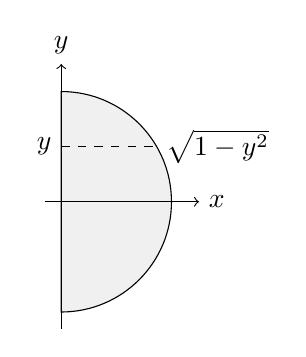
\begin{tikzpicture}[scale=1.4]
\fill[gray!12] (0,-1) arc[start angle=-90,end angle=90,radius=1] --cycle;
\draw (0,-1) arc[start angle=-90,end angle=90,radius=1] --cycle;
\draw[->] (-.15,0)--(1.25,0) node[right]{$x$};\draw[->] (0,-1.15)--(0,1.25) node[above]{$y$};
\draw[dashed] (0,.5)--(.866,.5);\node[left] at (0,.5){$y$};\node[right] at (.866,.5){$\sqrt{1-y^2}$};
\end{tikzpicture}\end{center}
虚线是条件 $Y=y$ 所对应的截面, 图仅展示积分区域.
\end{solution}

\begin{exercise}\label{ex:fl17-8}
原卷第8题(10分). $X,Y,Z$ 独立且均为 $\Exp(1)$. 求(a) $2X+1$, (b) $X+Y+Z$, (c) $\min\{X,Y,Z\}$ 的密度.
\end{exercise}
\begin{solution}
(a)\label{sol:fl17-8-a} 逆变换给 $f(u)=\tfrac12\ee^{-(u-1)/2}$, $u\geq1$.
(b)\label{sol:fl17-8-b} 先卷积两项得 $f_{X+Y}(u)=\int_0^u\ee^{-v}\ee^{-(u-v)}\dd v=u\ee^{-u}$. 再卷积一项得 $f_{X+Y+Z}(u)=\ee^{-u}\int_0^u v\dd v=u^2\ee^{-u}/2$, $u\geq0$.
(c)\label{sol:fl17-8-c} 最小值超过 $u\geq0$ 当且仅当三者都超过 $u$, 独立性给生存函数 $\ee^{-3u}$. 对 $1-\ee^{-3u}$ 求导, 密度 $3\ee^{-3u}$.
\end{solution}

\begin{exercise}\label{ex:fl17-9}
原卷第9题(10分). 猴子所在梯阶为0至7, 0表示地面. 在阶 $0\leq m\leq6$, 下一秒各以 $1/2$ 概率升到 $m+1$ 或落回0; 在7则下一秒必回0. (a) 给8阶转移矩阵, 可仅列非零项. (b) 从0出发, 七秒后位于7的概率是多少? (c) 求长期各阶时间比例 $(\pi_0,\ldots,\pi_7)$; 提示先比较 $\pi_j$ 和 $\pi_{j+1}$.
\end{exercise}
\begin{solution}
(a)\label{sol:fl17-9-a} 行为当前阶, 列为下一阶, 非零项为 $P_{m0}=P_{m,m+1}=1/2$ ($0\leq m\leq6$), $P_{70}=1$. 这也完整指定了官方矩阵.
(b)\label{sol:fl17-9-b} 七步到7必须连升七次, 有一次回落都来不及补足. 概率 $2^{-7}=1/128$.
(c)\label{sol:fl17-9-c} 每个 $j\geq1$ 只从 $j-1$ 获得流入, 平稳方程为 $\pi_j=\pi_{j-1}/2$. 故 $\pi_j=2^{7-j}\pi_7$, 归一化用 $1+2+\cdots+128=255$, 得 $\pi_j=2^{7-j}/255$. 第0列方程也满足, 因为全部流出总质量为1且其他列已平衡. 有限链不可约, 因而其长期时间比例为此唯一平稳分布.
\end{solution}

\begin{exercise}\label{ex:fl17-10}
原卷第10题(10分). $X_1,\ldots,X_{300}$ 独立且均匀于 $[0,100]$, $S=\sum_{i=1}^{300}X_i$. (a) 求均值、方差. (b) 用Poisson近似求恰有三个 $j$ 满足 $3\leq X_j<4$ 的概率. (c) 给区间 $[a,b]$, 中点为 $\E S$, 且 $\Prob(S\in[a,b])\approx.95$. 可用 $\int_{-2}^2\ee^{-x^2/2}\dd x/\sqrt{2\pi}\approx.95$.
\end{exercise}
\begin{solution}
(a)\label{sol:fl17-10-a} 单项均值50, 方差 $100^2/12$, 故 $\E S=15000$, $\Var S=300\cdot10000/12=250000$. 官方均值行写成 $100\E X_1=15000$, 其100应为300.
(b)\label{sol:fl17-10-b} 计数严格服从 $\Bin(300,.01)$, 以均值3的Poisson近似, 得 $\ee^{-3}3^3/3!=9/(2\ee^3)$.
(c)\label{sol:fl17-10-c} 标准差500, CLT把中心两标准差区间近似为正态的 $[-2,2]$. 可取 $[14000,16000]$. 这是正态近似, 不是有限样本的精确95\%保证.
\end{solution}

\originalsection{2018年春季期末卷}
本节对应\href{https://ocw.mit.edu/courses/18-600-probability-and-random-variables-fall-2019/resources/mit18_600f19_final_2018/}{官方题卷}与\href{https://ocw.mit.edu/courses/18-600-probability-and-random-variables-fall-2019/resources/mit18_600f19_final_2018_soln/}{官方解答}. 全卷100分, 每题10分; 解答依据官方解答重构, 补齐推导.

\begin{exercise}\label{ex:fl18-1}
原卷第1题. $(X,Y)$ 均匀分布在单位圆盘 $x^2+y^2\leq1$. (a) 给联合密度 $f(x,y)$. (b) 求边缘密度 $f_X$. (c) 把 $\E[X^2\mid Y]$ 写为 $Y$ 的函数.
\end{exercise}
\begin{solution}
(a)\label{sol:fl18-1-a} 圆盘面积 $\pi$, 故 $f(x,y)=\pi^{-1}\ind_{\{x^2+y^2\leq1\}}$.
(b)\label{sol:fl18-1-b} 固定 $|x|<1$, 竖直截面长度 $2\sqrt{1-x^2}$, 积分得 $f_X(x)=2\sqrt{1-x^2}/\pi$; $|x|>1$ 时为零.
(c)\label{sol:fl18-1-c} 给定 $Y=y$, $X$ 均匀于 $[-a,a]$, $a=\sqrt{1-y^2}$. 二阶矩为 $(2a)^{-1}\int_{-a}^a x^2\dd x=a^2/3$. 因而 $\E[X^2\mid Y]=(1-Y^2)/3$ 几乎处处, 边界版本不影响结论.
\end{solution}

\begin{exercise}\label{ex:fl18-2}
原卷第2题. Ivan等车, 黄、蓝、红车到达是三个独立Poisson点过程, 每小时平均分别3、2、1辆. (a) 首辆任意颜色车到达的等待时间 $T$ 有什么密度? (b) 首半小时恰好两辆黄车的概率? (c) 黄车接上后30分钟到家, 蓝或红车接上后15分钟到家. 若黄车先到, 为使到家总时间期望最小, 应上黄车还是等蓝红? 解释理由.
\end{exercise}
\begin{solution}
(a)\label{sol:fl18-2-a} 时间以小时计. 三者在 $[0,t]$ 都无到达的概率为 $\ee^{-3t}\ee^{-2t}\ee^{-t}=\ee^{-6t}$, 因而 $f_T(t)=6\ee^{-6t}$, $t\geq0$.
(b)\label{sol:fl18-2-b} 黄车计数为 $\Pois(3/2)$, 故概率为 $\ee^{-3/2}(3/2)^2/2!$.
(c)\label{sol:fl18-2-c} 从黄车到达时刻重新计时, 独立增量与无记忆性保证蓝红剩余等待仍为率3的指数变量, 均值 $1/3$ 小时即20分钟. 等蓝红的总期望为 $20+15=35$ 分钟; 立即上黄车为30分钟. 已经过的等待对两策略相同, 所以应上黄车.
\end{solution}

\begin{exercise}\label{ex:fl18-3}
原卷第3题. 房地产经纪人Harriet与Helen每周各尝试成交一单, 强者成功率 $.2$, 弱者 $.1$. 强者第 $j$ 周的指示变量为 $X_j$, 弱者为 $Y_j$, 所有变量相互独立. 令 $Z_j=X_j-Y_j$, $S_n=\sum_{j=1}^nZ_j$. (a) 求 $Z_1$ 的均值、方差、标准差. (b) 求 $S_{100}$ 的对应三量. (c) 用CLT近似 $\Prob(S_{100}>0)$, 可以用 $\Phi$ 表示.
\end{exercise}
\begin{solution}
(a)\label{sol:fl18-3-a} 差的均值 $.2-.1=.1$. 独立性使方差相加, $\Var Z_1=.2(.8)+.1(.9)=.25$, 标准差 $.5$.
(b)\label{sol:fl18-3-b} $Z_j$ 独立同分布, 所以 $\E S_{100}=10$, $\Var S_{100}=25$, 标准差5.
(c)\label{sol:fl18-3-c} 标准化门槛 $(0-10)/5=-2$, 故 $\Prob(S_{100}>0)\approx1-\Phi(-2)=\Phi(2)\approx.9772$. 这按原卷采用不作连续性修正的CLT近似; 整数格点修正可给不同的有限样本近似, 并非改变精确事件.
\end{solution}

\begin{exercise}\label{ex:fl18-4}
原卷第4题. 社会有7家公司, 软件工程师每月底状态为失业0或公司 $j\in\{1,\ldots,7\}$. 失业者次月以 $3/10$ 概率仍失业, 以各 $1/10$ 概率去每家公司; 公司 $j$ 员工以 $69/70$ 留在原公司, 以 $1/70$ 失业. (a) 给8阶矩阵非零项. (b) 当前失业, 两个月后仍失业的概率? (c) 求长期状态比例 $(\pi_0,\ldots,\pi_7)$, 提示先求 $\pi_0$.
\end{exercise}
\begin{solution}
(a)\label{sol:fl18-4-a} 非零项为 $P_{00}=3/10$, $P_{0j}=1/10$, $P_{j0}=1/70$, $P_{jj}=69/70$ ($1\leq j\leq7$). 行和均为1.
(b)\label{sol:fl18-4-b} 中间时刻或失业或去某公司, 故 $P^2_{00}=(3/10)^2+7(1/10)(1/70)=1/10$.
(c)\label{sol:fl18-4-c} 把七家公司合成就业状态 $E$, 转移只取决于就业/失业, 仍为二态Markov链. 平衡流 $\pi_U(7/10)=\pi_E(1/70)$ 给 $\pi_E=49\pi_U$, 所以 $\pi_U=1/50=.02$. 每家公司对称且链不可约, 故 $\pi_j=.98/7=.14$; 也可由 $\pi_j/70=\pi_0/10$ 逐一核验.
\end{solution}

\begin{exercise}\label{ex:fl18-5}
原卷第5题. 烤面包机客服电话来电分7类: 买新机、轻档仍太焦各 $1/4$; 联网失败、手卡住、起火各 $1/8$; 询问肉桂吐司、调弹簧使吐司飞高各 $1/16$. 下一位类别为 $X$. (a) 求 $H(X)$. (b) 最优是非问题策略的平均询问次数? (c) 一天100次来电类别 $X_1,\ldots,X_{100}$ 独立且与 $X$ 同分布, 求联合熵. (d) $Y$ 是购买新机人数, $Z=Y^2$, 求 $H(Z)$, 可写求和式.
\end{exercise}
\begin{solution}
(a)\label{sol:fl18-5-a} $H(X)=2(1/4)2+3(1/8)3+2(1/16)4=21/8$.
(b)\label{sol:fl18-5-b} 取前缀码 $00,01,100,101,110,1110,1111$. 平均长度等于(a)的熵 $21/8$, 而编码熵下界保证不可更小. 各码对应七类来电, 按位提问就是具体策略.
(c)\label{sol:fl18-5-c} 独立联合熵相加, 得 $100(21/8)=525/2$.
(d)\label{sol:fl18-5-d} $Y\sim\Bin(100,1/4)$, 非负整数集合上平方是单射, 所以 $Z$ 只是把结果重新命名, 熵不变. 若 $p_k=\binom{100}k(1/4)^k(3/4)^{100-k}$, 则 $H(Z)=H(Y)=-\sum_{k=0}^{100}p_k\log_2p_k$. 此式给全分布而不需大数近似.
\end{solution}

\begin{exercise}\label{ex:fl18-6}
原卷第6题. $X_i$ 独立标准Cauchy变量, 密度 $1/[\pi(1+x^2)]$. $S_0=0$, $S_n=\sum_{j=1}^nX_j$. (a) $S_n$ 是否为鞅? 明确核查鞅定义中的 $\E|S_n|<\infty$. (b) 求 $S_{10}$ 密度. (c) 求 $\Prob(S_{10}>10)$.
\end{exercise}
\begin{solution}
(a)\label{sol:fl18-6-a} 已在 $n=1$ 失去可积性, 因 $\E|X_1|=(2/\pi)\int_0^\infty x/(1+x^2)\dd x=\infty$. 所以不论形式上的对称性如何, $S_n$ 不是鞅; 不能把对称主值0当作期望.
(b)\label{sol:fl18-6-b} Cauchy稳定性给 $S_{10}\overset d=10X_1$, 变换密度为 $1/[10\pi(1+(x/10)^2)]$.
(c)\label{sol:fl18-6-c} 所求等于 $\Prob(X_1>1)=1/2-\arctan(1)/\pi=1/4$.
\end{solution}

\begin{exercise}\label{ex:fl18-7}
原卷第7题. 独立 $X_i$ 各以 $1/2$ 概率取 $-2,2$, $S_0=0$, $S_n=\sum_{j=1}^nX_j$. (a) 先到20而非 $-30$ 的概率? (b) 存在正整数 $n$ 使 $S_n=-20$ 的概率? (c) 求 $M_{X_1}(t)$. (d) 求 $M_{S_9}(t)$.
\end{exercise}
\begin{solution}
(a)\label{sol:fl18-7-a} 这是可积零均值独立增量鞅. 首次退出有限格点区间的停时几乎必然有限, 且停止值有界, 如2017年题\ref{ex:fl17-4}的论证. 若 $p$ 为先20概率, $0=20p-30(1-p)$, 故 $p=3/5$.
(b)\label{sol:fl18-7-b} 对任意正偶数 $K$, 先到 $-20$ 而非 $K$ 的概率由同一方程为 $K/(K+20)$. 这是最终曾到 $-20$ 的下界, 令偶数 $K\to\infty$ 下界趋1, 概率不能超过1, 因而答案1. 不对无界的最终击中停时直接套有界停止定理.
(c)\label{sol:fl18-7-c} 直接按二点分布求期望: $M_{X_1}(t)=(\ee^{2t}+\ee^{-2t})/2$.
(d)\label{sol:fl18-7-d} 指数把和化为积, 独立性把期望化为乘积, 得 $M_{S_9}(t)=[(\ee^{2t}+\ee^{-2t})/2]^9$.
\end{solution}

\begin{exercise}\label{ex:fl18-8}
原卷第8题. 1至6号牌均匀随机排列, 依次翻牌; 新牌大于此前所有牌时喊``纪录'', 首张自动算纪录. 例如递增排列有6次, 顺序 $6,3,4,5,1,2$ 只有1次. $A_i$ 表示第 $i$ 张是否纪录, $R=\sum A_i$. (a) 求 $\E R$. (b) 求 $\Var R$. (c) 给定前三张都为纪录, 后三张也全为纪录的条件概率?
\end{exercise}
\begin{solution}
(a)\label{sol:fl18-8-a} 前 $i$ 个值最大者的位置均匀, 所以 $\Prob(A_i=1)=1/i$, 得 $\E R=\sum_{i=1}^6 1/i=49/20$.
(b)\label{sol:fl18-8-b} 为说明独立性, 令 $J_i$ 为第 $i$ 个值在前 $i$ 个值中的相对名次. 每个排列唯一对应一串 $J_i\in\{1,\ldots,i\}$: 倒着逐次移去相应名次即可重建排列. 此类名次串共 $\prod_{i=1}^6i=6!$ 种, 均匀排列使每串等概率, 故 $J_i$ 相互独立且各均匀. $A_i=\ind_{\{J_i=i\}}$ 因而独立. 所以
\[\Var R=\sum_{i=1}^6\frac1i\left(1-\frac1i\right)
=\frac14+\frac29+\frac3{16}+\frac4{25}+\frac5{36}=\frac{3451}{3600}.\]
(c)\label{sol:fl18-8-c} 六次全纪录即唯一的递增排列, 概率 $1/6!$; 前三张递增概率 $1/3!$. 前者包含于后者, 比值为 $3!/6!=1/120$.
\end{solution}

\begin{exercise}\label{ex:fl18-9}
原卷第9题. $X_1,X_2,\ldots$ 独立标准正态. (a) 序列 $X_n$ 是否为鞅? 一句话解释. (b) $A=\sum_{n=1}^{60}X_n$, $B=\sum_{n=41}^{100}X_n$, 求相关系数. (c) 写 $A$ 密度. (d) 求 $\Var(A+B)$.
\end{exercise}
\begin{solution}
(a)\label{sol:fl18-9-a} 不是: 在自然过滤 $\mathcal F_{n-1}$ 下, 可积的 $X_n$ 因独立性有条件均值0, 而 $X_{n-1}$ 几乎必然不等于0.
(b)\label{sol:fl18-9-b} 两和各有60项, 方差均60. 协方差双和中只有同指标项留下, 重叠指标41至60共20个, 得 $\Cov(A,B)=20$, 所以相关为 $20/60=1/3$.
(c)\label{sol:fl18-9-c} 独立正态之和为 $\Normal(0,60)$, 密度 $f_A(x)=\ee^{-x^2/120}/\sqrt{120\pi}$.
(d)\label{sol:fl18-9-d} 两和并不独立, 方差应加上交叉项, 得 $60+60+2\cdot20=160$.
\end{solution}

\begin{exercise}\label{ex:fl18-10}
原卷第10题. $X,Y,Z$ 独立且均为 $\Exp(1)$. (a) 求三者和的密度. (b) 求三者最大值的均值与方差. (c) 求最小值的均值与方差.
\end{exercise}
\begin{solution}
(a)\label{sol:fl18-10-a} 卷积推导见题\ref{ex:fl17-8}(b), 得 $u^2\ee^{-u}/2$, $u\geq0$.
(b)\label{sol:fl18-10-b} 将三个指数时钟看作三件独立物品的失效时间. 首次失效间隔为 $\Exp(3)$; 给定首失效, 剩余两时钟因无记忆性重启, 第二间隔为独立 $\Exp(2)$; 最后间隔为独立 $\Exp(1)$. 这里每阶段剩余时间的条件联合分布不依赖过去, 故间隔独立. 最大值是这三间隔之和, 均值 $1/3+1/2+1=11/6$, 方差 $1/9+1/4+1=49/36$.
(c)\label{sol:fl18-10-c} 最小值为 $\Exp(3)$, 因三生存函数相乘为 $\ee^{-3u}$. 因而均值 $1/3$, 方差 $1/9$.
\end{solution}

\originalsection{2019年春季期末卷}
本节对应\href{https://ocw.mit.edu/courses/18-600-probability-and-random-variables-fall-2019/resources/mit18_600f19_final_2019/}{官方题卷}与\href{https://ocw.mit.edu/courses/18-600-probability-and-random-variables-fall-2019/resources/mit18_600f19_final_2019_soln/}{官方解答}. 全卷100分, 每题10分; 解答依据官方解答重构, 补齐推导.

\begin{exercise}\label{ex:fl19-1}
原卷第1题. 西兰花商人选网页图片: 图1为漂亮的人在海滩吃西兰花, 图2为西兰花配三文鱼和藜麦特写. 较有效图对应访客消费均值16美元, 较差图为14美元, 两者标准差都10美元. A/B试验各向50人展示一图. 记有效图消费 $X_1,\ldots,X_{50}$, 差图消费 $Y_1,\ldots,Y_{50}$, 两组内部同分布, 全100变量独立, $\E X_i=16$, $\E Y_i=14$, $\Var X_i=\Var Y_i=100$. $X=\sum X_i$, $Y=\sum Y_i$. (a) 用CLT近似 $\Prob(X>Y)$, 可用 $\Phi$. (b) 将 $\E[(X_1-Y_1)\mid X]$ 写成 $X$ 的函数. (c) 求 $\E[(X-Y)^2]$.
\end{exercise}
\begin{solution}
(a)\label{sol:fl19-1-a} 配对差 $D_i=X_i-Y_i$ 独立同分布, 均值2, 方差200. 因而总差均值100、方差 $50\cdot200=10000$、标准差100. 标准化零门槛为 $-1$, 故 $\Prob(X>Y)\approx1-\Phi(-1)=\Phi(1)\approx.8413$. 官方把 $50\cdot100+50\cdot100$ 写成100000, 正确值10000; 其标准差100和最终近似正确. 官方等式链中的 $1-\Phi(-1)-\Phi(1)$ 也应改为 $1-\Phi(-1)=\Phi(1)$.
(b)\label{sol:fl19-1-b} 由于 $X_i$ 交换对称, 所有 $\E[X_i\mid X]$ 相同; 又其和为 $\E[X\mid X]=X$, 得每项为 $X/50$. $Y_1$ 独立于 $X$, 故 $\E[Y_1\mid X]=14$. 所求 $X/50-14$.
(c)\label{sol:fl19-1-c} 二阶矩为方差加均值平方, 得 $10000+100^2=20000$.
\end{solution}

\begin{exercise}\label{ex:fl19-2}
原卷第2题. 探险者遇到10个岛民, 每人有10个苹果. 每步(i)均匀选 $\binom{10}2$ 对中的一对; (ii)若两人都有苹果, 公平掷币决定赢家, 由输家向赢家转移1苹果; 若任一人没有苹果, 则不动. 重复直到一个总赢家有全部100苹果, 给定此事几乎必然发生, 不必证明. 第 $j$ 人在 $n$ 步后苹果数为 $A_n^j$, 结束时刻 $T$, $A_0^j=10$, $A_T^j$ 为赢家时100否则0. (a) 固定 $j$, $A_n^j$ 是否鞅? 解释. (b) 曾有恰好25苹果的人数期望? (c) 从未有超过10苹果的人数期望? (d) 总赢家曾只剩1苹果的概率? 提示事件 $B_j$ 为第 $j$ 人先降到1再升到100, 各 $B_j$ 互斥.
\end{exercise}
\begin{solution}
(a)\label{sol:fl19-2-a} 过滤包含各步配对、币值和所有苹果数. $0\leq A_n^j\leq100$ 保证可积与适应. 给定历史, 除非 $j$ 被选入且两方都有苹果, 否则增量为零; 若能转移, $+1,-1$ 等概率, 条件均值为零. 因此是鞅, 结束后保持不动.
(b)\label{sol:fl19-2-b} 首次 $A_n^j\in\{0,25\}$ 的停时 $S$ 在结束前必发生, 因增量最多1, 从10到100必须经过25; 故 $S\leq T<\infty$ 几乎必然. 停止过程在 $[0,25]$ 内, 可选停止与有界收敛给 $10=25\Prob(A_S^j=25)$, 所以每人概率 $.4$. 人数为十个指示变量之和, 期望4.
(c)\label{sol:fl19-2-c} 将(b)上界换成11. 曾超过10即先到11而非0, 概率 $10/11$; 从未超过10概率 $1/11$, 人数期望 $10/11$.
(d)\label{sol:fl19-2-d} 先到1而非100概率由 $10=1p+100(1-p)$ 得 $p=90/99=10/11$. 在首次到1的历史上, 再用有界鞅停止于0或100, 最终该人获胜的条件概率为 $1/100$. 这一步只需条件公平性, 不需把苹果数单独假设成Markov链. 故 $\Prob(B_j)=1/110$. 赢家唯一使事件互斥, 十项相加得到 $1/11$.
\end{solution}

\begin{exercise}\label{ex:fl19-3}
原卷第3题. Irene审讯有罪者时供认概率 $.9$, 无罪者为 $.1$; 她的技巧包括隔离与声称供认有利, 故可能有虚假供认. 10人中恰1人有罪. 每天独立均匀选1人审讯, 可重复同一人, 各次供认在给定所选者罪责后独立且概率固定. 首次有人供认即结案并拘禁该人. (a) 首日获得供认概率? (b) 给定首日供认, 被审者有罪概率? (c) $N$ 为总审讯次数(含最后一次), 求 $\Prob(N=k)$, $k\geq1$, 及 $\E N$. (d) 最终拘禁者有罪的概率?
\end{exercise}
\begin{solution}
(a)\label{sol:fl19-3-a} 全概率为 $(1/10)(.9)+(9/10)(.1)=.18$.
(b)\label{sol:fl19-3-b} 有罪且供认概率 $.09$, 除以 $.18$ 得 $1/2$.
(c)\label{sol:fl19-3-c} 每日新的随机选择与供认试验使是否供认独立, 成功率 $.18$. 故 $N\sim\Geom(.18)$ (从1起), $\Prob(N=k)=(.82)^{k-1}(.18)$, $\E N=1/.18=50/9$.
(d)\label{sol:fl19-3-d} 对任何结束日 $k$, 前 $k-1$ 日无供认独立于当天的试验; 当天给定供认, 有罪概率仍 $1/2$. 对所有 $k$ 按 $\Prob(N=k)$ 加权, 结果 $1/2$. 不能把``重复审讯直到供认''当作消除虚假供认的方法.
\end{solution}

\begin{exercise}\label{ex:fl19-4}
原卷第4题. 8人把帽子放入箱中, 均匀随机打乱后每人取回1帽; 每帽在箱中又以 $1/2$ 概率独立于一切其他随机性落入泥角变脏. (a) $D$ 为脏帽数, 求均值和方差. (b) $N$ 为拿回自己帽子的人数, $N^*$ 为拿回自己且干净帽子的人数. 可用指示变量 $N_i^*$, $N^*=\sum_{i=1}^8N_i^*$. 求 $N^*$ 均值方差. (c) $C$ 为干净帽数, 求 $\rho(C,D)$ 与 $\rho(N,C)$; 提示无需大量计算.
\end{exercise}
\begin{solution}
(a)\label{sol:fl19-4-a} $D\sim\Bin(8,1/2)$, 故均值4、方差2.
(b)\label{sol:fl19-4-b} $\Prob(N_i^*=1)=1/(8\cdot2)=1/16$, 故 $\E N^*=1/2$. 对 $i\ne j$, 两人都拿回自己帽概率 $(1/8)(1/7)=1/56$, 两帽同时干净概率 $1/4$, 所以 $\E(N_i^*N_j^*)=1/224$. 展开平方中有8个对角项与56个有序非对角项:
\[\E[(N^*)^2]=8/16+56/224=3/4,\qquad\Var N^*=3/4-(1/2)^2=1/2.\]
官方某行写作 $\E[N^*]^2$, 该位置实际需要的是 $\E[(N^*)^2]$.
(c)\label{sol:fl19-4-c} $D=8-C$, 两方差非零且完全反向线性, 故 $\rho(C,D)=-1$. $N$ 只由随机排列决定, $C$ 只由独立的脏净试验决定, 所以独立且相关为0.
\end{solution}

\begin{exercise}\label{ex:fl19-5}
原卷第5题. 生物技术公司员工等级1至5, 每年末重分: 1至4级各以 $1/2$ 留原级、$1/2$ 晋一级; 5级必回1级, 体现公司宣称的``回归基层''. (a) 写转移矩阵. (b) 求长期各等级比例. (c) 从 $A_0=1$ 出发, 求首次到5级的期望年数 $\E\min\{n:A_n=5\}$.
\end{exercise}
\begin{solution}
(a)\label{sol:fl19-5-a} 按1至5排序,
\[P=\begin{pmatrix}1/2&1/2&0&0&0\\0&1/2&1/2&0&0\\0&0&1/2&1/2&0\\0&0&0&1/2&1/2\\1&0&0&0&0\end{pmatrix}.\]
(b)\label{sol:fl19-5-b} 2至4列方程为 $\pi_j=\pi_j/2+\pi_{j-1}/2$, 故前四项相同; 第5列给 $\pi_5=\pi_4/2$. 归一化得到 $(2,2,2,2,1)/9$. 第1列 $\pi_1=\pi_1/2+\pi_5$ 同样满足. 链有限不可约, 此为长期时间比例.
(c)\label{sol:fl19-5-c} 每级晋升等待是从1起的 $\Geom(1/2)$, 均值2. 首次到5只需四次晋升, 无向下转移, 所以四段等待期望相加为8年; 期望线性本身不要求这些等待独立.
\end{solution}

\begin{exercise}\label{ex:fl19-6}
原卷第6题. $X$ 均匀于 $[0,10]$, 对实数 $K$ 令 $C(K)=\E\max\{X-K,0\}$. (a) 求 $0\leq K\leq10$ 的 $C(K)$, 提示积分是三角形面积. (b) 求区间上的 $C',C''$. (c) 求 $\E X^3$.
\end{exercise}
\begin{solution}
(a)\label{sol:fl19-6-a} 只有 $x>K$ 有收益, 因而 $C(K)=\int_K^{10}(x-K)\dd x/10=(10-K)^2/20$. 几何上这是底与高都为 $10-K$ 的三角形面积除以10.
(b)\label{sol:fl19-6-b} 在内部 $0<K<10$, $C'(K)=K/10-1$, $C''(K)=1/10$. 原题写``区间上'', 端点按内侧导数可延用这些值; 若把 $C$ 定义在全实轴, $K<0$ 时 $C=5-K$, $K>10$ 时 $C=0$, 一阶导连续但两端二阶导数不存在. 这一区别不能被多项式形式掩盖.
(c)\label{sol:fl19-6-c} $\E X^3=(1/10)\int_0^{10}x^3\dd x=250$.
\end{solution}

\begin{exercise}\label{ex:fl19-7}
原卷第7题. $X_1,X_2,\ldots$ 独立且均为 $\Exp(1)$. (a) $c$ 固定, $Y_n=(\sum_{i=1}^nX_i^3)-cn$, $Y_0=0$. 哪些 $c$ 使它为鞅? (b) 求 $\Prob(X_1+X_2+X_3<2,\ X_1+X_2+X_3+X_4>2)$, 提示作Poisson点过程解释. (c) 求 $\rho(X_1+X_2+X_3,X_2+X_3+X_4)$. (d) 给三项和密度.
\end{exercise}
\begin{solution}
(a)\label{sol:fl19-7-a} PDF原式是立方之和, 并非和的立方. 对 $\mathcal F_n=\sigma(X_1,\ldots,X_n)$, 适应性成立, 而 $\E X_i^3=3!=6$ 保证固定时刻可积. 条件增量均值 $\E(X_{n+1}^3-c)=6-c$, 所以充要条件 $c=6$.
(b)\label{sol:fl19-7-b} 相邻到达间隔为独立 $\Exp(1)$ 的累计和组成率1的Poisson点过程. 题述事件恰是 $[0,2]$ 有3点, 到达恰等于2的概率零. 计数为 $\Pois(2)$, 故答案 $\ee^{-2}2^3/3!=4\ee^{-2}/3$.
(c)\label{sol:fl19-7-c} 单项方差1, 两和方差各3, 重叠的 $X_2,X_3$ 给协方差2, 故相关 $2/3$.
(d)\label{sol:fl19-7-d} 卷积见题\ref{ex:fl17-8}(b), 得 $x^2\ee^{-x}/2$, $x\geq0$.
\end{solution}

\begin{exercise}\label{ex:fl19-8}
原卷第8题. $(X,Y)$ 均匀于单位圆盘 $x^2+y^2\leq1$. (a) 求联合密度. (b) 求 $X$ 的边缘密度. (c) $R=\sqrt{X^2+Y^2}$, 求 $\E R$, 提示极坐标积分或先求 $F_R,f_R$.
\end{exercise}
\begin{solution}
(a)\label{sol:fl19-8-a} 与题\ref{ex:fl18-1}(a)条件和所求完全相同, 密度为圆盘内 $1/\pi$, 盘外零.
(b)\label{sol:fl19-8-b} 同题\ref{ex:fl18-1}(b), $f_X(x)=2\sqrt{1-x^2}/\pi$ ($|x|\leq1$).
(c)\label{sol:fl19-8-c} $0\leq r\leq1$ 时, 半径不超过 $r$ 的子盘面积占比 $\pi r^2/\pi=r^2$. 故 $F_R(r)=r^2$, 密度 $2r$, 于是 $\E R=\int_0^1r(2r)\dd r=2/3$.
\end{solution}

\begin{exercise}\label{ex:fl19-9}
原卷第9题. Andrew与Alyssa逐个生孩子, 到首次同时有男孩女孩或已有4个孩子时停止. 性别序列 $X$ 的可能值为 $\{GB,GGB,GGGB,GGGG,BG,BBG,BBBG,BBBB\}$. 每个孩子独立以 $.5$ 为女孩G或男孩B. (a) 求 $H(X)$ 的具体有理数. (b) 描述一系列是非问题, 使确定 $X$ 的平均问题数恰等于 $H(X)$. (c) $Y\in\{G,B\}$ 为首孩性别, 求 $H(Y),H_Y(X),H(X,Y)$, 并判断 $H(X,Y)=H(Y)+H_Y(X)$.
\end{exercise}
\begin{solution}
(a)\label{sol:fl19-9-a} 长度2的两结果各概率 $1/4$, 长度3的两结果各 $1/8$, 长度4的四结果各 $1/16$. 结果负对数恰是长度, 得熵 $(1/2)2+(1/4)3+(1/4)4=11/4$.
(b)\label{sol:fl19-9-b} 逐次问``第一个孩子是女孩吗?'', ``第二个呢?''等, 一旦男女都出现或已问4次即停. 每个未结束节点的下个性别仍公平, 该树叶就是可能的 $X$. 问题数等于序列长度, 平均 $11/4$, 达到熵下界.
(c)\label{sol:fl19-9-c} 首孩公平所以 $H(Y)=1$. 给定G时四种序列的条件概率为 $1/2,1/4,1/8,1/8$, 熵为 $(1/2)1+(1/4)2+2(1/8)3=7/4$; 给定B相同, 所以 $H_Y(X)=7/4$. $X$ 唯一确定 $Y$, 对 $(X,Y)$ 的结果重新命名不改变概率, 故联合熵 $11/4=1+7/4$, 恒等式成立.
\end{solution}

\begin{exercise}\label{ex:fl19-10}
原卷第10题. $X_1,\ldots,X_5$ 独立标准Cauchy, 密度 $1/[\pi(1+x^2)]$. (a) 求 $\Prob(\max(X_1,X_2)>\max(X_3,X_4,X_5))$. (b) $N$ 是五项中正值个数, 求 $M_N(t)$. (c) 求 $\Prob(X_1+X_2>X_3+X_4+X_5+5)$.
\end{exercise}
\begin{solution}
(a)\label{sol:fl19-10-a} 连续独立分布使并列最大概率零, 五个位置对称, 其中最大在前两个的概率 $2/5$.
(b)\label{sol:fl19-10-b} 对称性给单项正值概率 $1/2$, 指示变量独立, $N\sim\Bin(5,1/2)$. 因而 $M_N(t)=[(1+\ee^t)/2]^5$.
(c)\label{sol:fl19-10-c} 对称性使负号Cauchy与正号同分布, 且独立性不变. 差 $X_1+X_2-X_3-X_4-X_5$ 的特征函数为 $\ee^{-5|t|}$, 与 $5X_1$ 相同. 因此概率 $\Prob(5X_1>5)=\Prob(X_1>1)=1/4$.
\end{solution}

\originalsection{2019年秋季期末卷}
本节对应\href{https://ocw.mit.edu/courses/18-600-probability-and-random-variables-fall-2019/resources/mit18_600f19_final_f2019/}{官方题卷}与\href{https://ocw.mit.edu/courses/18-600-probability-and-random-variables-fall-2019/resources/mit18_600f19_final_f2019_soln/}{官方解答}. 全卷100分. 题1、2、5至10各标10分, 题3、4未印分值; 解答依据官方解答重构, 补齐推导.

\begin{exercise}\label{ex:flf19-1}
原卷第1题. 60学生, 男孩女孩各30人, 均匀随机分成各30人的班1和班2, $\binom{60}{30}$ 种班1选择等可能. 校长告知班1至少29个女孩. 家长0问是否全30人都是女孩; 家长1认为概率 $1/2$, 因每个孩子为女孩概率 $1/2$; 家长2认为已知29女孩后余31人仅1女孩, 应为 $1/31$; 家长3认为两人都错, 概率更小. (a) 事件 $A$ 为班1全女孩, $B$ 为至少29女孩, 求 $\Prob A,\Prob B$. (b) 求 $\Prob(A\mid B)$, 判断谁正确. (c) $G$ 和 $B$ 此处改表示班1女生、男生人数, 求 $\E[GB]$.
\end{exercise}
\begin{solution}
(a)\label{sol:flf19-1-a} 全女仅一种选择, $\Prob A=1/\binom{60}{30}$. 恰29女孩时选遗漏女孩有30种, 入班男孩有30种, 共900种, 故 $\Prob B=901/\binom{60}{30}$.
(b)\label{sol:flf19-1-b} $A\subset B$, 条件概率为比值 $1/901$, 家长3正确. 条件``至少29女孩''不是按顺序观察到29个女孩后再抽第30个, 后一种条件才会导向家长2的计算; 题中给定的是全班性别人数事件.
(c)\label{sol:flf19-1-c} 令 $G_i,B_j$ 为指定女孩、男孩是否进班1的指示变量, 则 $GB=\sum_{i,j=1}^{30}G_iB_j$. 一对指定学生都进班1概率 $(30/60)(29/59)$, 故 $\E[GB]=900(1/2)(29/59)=13050/59$.
\end{solution}

\begin{exercise}\label{ex:flf19-2}
原卷第2题. 三岁孩子申请两所选择性幼儿园, 两次入学考试测量技能但有噪声. 分数 $S_1=A+2B_1$, $S_2=A+2B_2$, $A,B_1,B_2$ 独立标准正态; $A$ 表示能力, $B_i$ 为噪声. (a) 求 $\E[S_1S_2]$. (b) 求两方差与相关系数. (c) 把 $\E[S_2\mid S_1]$ 写成 $S_1$ 的函数. 提示 $2B_1$ 与四个独立标准正态之和同分布.
\end{exercise}
\begin{solution}
(a)\label{sol:flf19-2-a} 展开为 $A^2+2AB_1+2AB_2+4B_1B_2$. 混合项独立且零均值, 只有 $\E A^2=1$ 留下.
(b)\label{sol:flf19-2-b} 每分数方差 $1+4=5$, 均值0, 故协方差为(a)的1, 相关 $1/5$. 官方将第二方差的变量偶写为 $B_2$, 这里所求为 $S_2$.
(c)\label{sol:flf19-2-c} $B_2$ 独立于 $S_1$, 条件均值为零, 故只求 $\E[A\mid A+2B_1]$. 按提示把 $(A,2B_1)$ 的联合分布等价写成 $(Y_0,Y_1+\cdots+Y_4)$, $Y_i$ 独立标准正态. 给定总和 $S=\sum_{i=0}^4Y_i$, 五项条件期望因交换对称相同, 相加为 $S$, 故各为 $S/5$. 因此 $\E[S_2\mid S_1]=S_1/5$. 这是联合分布的替换, 不声称原空间中 $2B_1$ 已经等于四个新变量之和.
\end{solution}

\begin{exercise}\label{ex:flf19-3}
原卷第3题. Jill热爱吉他, 每首歌16小节. 每小节独立随机选已会的5个和弦: A大调概率 $1/2$; F\#小调、D大调、B小调、E大调各 $1/8$. $X=(X_1,\ldots,X_{16})$ 为整歌和弦序列. (a) 求首和弦熵 $H(X_1)$. (b) 求整歌熵 $H(X)$. (c) 描述平均问题数最少的是非询问策略以确定 $X$, 并给平均数. (d) $S=\{i:X_i=\text{A大调}\}$ 为A和弦位置集合, 求 $H(S),H(S,X),H_S(X)$.
\end{exercise}
\begin{solution}
(a)\label{sol:flf19-3-a} $H(X_1)=(1/2)1+4(1/8)3=2$ 比特.
(b)\label{sol:flf19-3-b} 各小节独立, 联合熵 $16\cdot2=32$ 比特.
(c)\label{sol:flf19-3-c} 对每小节先问是否A大调; 若否, 对另外四和弦用两个二元问题编码, 例如问``是F\#小调或D大调吗?''与``是F\#小调或B小调吗?''. 四者的两回答组合各不同. 一半时候1问, 一半时候3问, 单节平均2, 整歌32. 熵下界保证最优.
(d)\label{sol:flf19-3-d} $S$ 对应16个独立公平的A/非A指示位, $H(S)=16$. $S$ 为 $X$ 的确定函数, 所以 $H(S,X)=H(X)=32$. 链式法则给 $H_S(X)=32-16=16$. 也可直接看给定 $S$ 后每个非A位置仍有四个等可能和弦, 单位置2比特, 平均非A位置8个, 得16.
\end{solution}

\begin{exercise}\label{ex:flf19-4}
原卷第4题. 小型技术大学只有人文、科学、工程、商科、数学5专业, 学生每周恰属一专业且经常转专业. 若本周数学, 下周以 $1/2$ 留数学, 以各 $1/8$ 去其他专业; 若本周非数学, 下周五专业各概率 $1/5$(包括原专业). (a) 写五阶转移矩阵. (b) 首周数学, 两周后为商科的概率? (c) 长期各专业时间比例?
\end{exercise}
\begin{solution}
(a)\label{sol:flf19-4-a} 按数学、人文、科学、工程、商科排序,
\[P=\begin{pmatrix}1/2&1/8&1/8&1/8&1/8\\1/5&1/5&1/5&1/5&1/5\\1/5&1/5&1/5&1/5&1/5\\1/5&1/5&1/5&1/5&1/5\\1/5&1/5&1/5&1/5&1/5\end{pmatrix}.\]
(b)\label{sol:flf19-4-b} 中间周数学概率 $1/2$, 非数学总概率 $1/2$. 所求 $(1/2)(1/8)+(1/2)(1/5)=13/80$.
(c)\label{sol:flf19-4-c} 其他四项对称为 $c$, 数学比例 $m=1-4c$. 数学列方程 $m=m/2+4c/5$, 得 $m=8c/5$. 与归一化联立得 $c=5/28$, $m=2/7$. 其余列核查为 $m/8+4c/5=c$. 有限不可约链保证长期比例是此平稳向量.
\end{solution}

\begin{exercise}\label{ex:flf19-5}
原卷第5题. $X\sim\Exp(1)$, 对实数 $K$ 定义 $C(K)=\E\max(X-K,0)$. (a) 求 $K\geq0$ 的 $C(K)$. (b) 求 $[0,\infty)$ 上两阶导数. (c) 求 $\E[X^3+3X^2+3X+1]$.
\end{exercise}
\begin{solution}
(a)\label{sol:flf19-5-a} 在积分中令 $u=x-K$, 得
\[C(K)=\int_K^\infty(x-K)\ee^{-x}\dd x
=\ee^{-K}\int_0^\infty u\ee^{-u}\dd u=\ee^{-K}.\]
(b)\label{sol:flf19-5-b} $K>0$ 时 $C'(K)=-\ee^{-K}$, $C''(K)=\ee^{-K}$. 在0取右侧导数也是该式. 全实轴定义下 $K<0$ 时 $C(K)=1-K$, 故0处一阶可导但二阶左右不一致.
(c)\label{sol:flf19-5-c} 指数整数矩 $\E X^k=k!$, 故结果 $3!+3\cdot2!+3\cdot1!+1=16$.
\end{solution}

\begin{exercise}\label{ex:flf19-6}
原卷第6题. 一个党派有100选民, 23候选编号1至23. 初始时每人恰支持一候选: 1至15各2票, 16至20各3票, 21号11票, 22号21票, 23号23票. 每单位时间均匀选 $\binom{100}2$ 对选民中的一对讨论. 若支持同人则不变; 否则公平币选其中一人转而支持另一人候选. 持续至时刻 $T$ 全体支持同一人, 该人获提名. 给定 $T<\infty$ 几乎必然, 不必证明. $A_i(t)$ 表示候选 $i$ 时刻 $t$ 的票数. (a) 各 $A_i(t)$ 是否鞅? (b) 23号曾在某 $0<t<T$ 仅有1票的概率? (c) $N$ 是曾在某 $0<t<T$ 仅1票的候选数, 求 $\E N$, 可用 $\sum_i(100-A_i(0))=2200$. (d) 获胜者曾仅有1票的``惊天逆转''概率?
\end{exercise}
\begin{solution}
(a)\label{sol:flf19-6-a} 取讨论历史过滤, 票数适应并被0和100夹住, 可积. 只有一人支持 $i$ 一人不支持时会变, 此时正负1各概率 $1/2$, 给定历史的增量期望零, 所以是鞅.
(b)\label{sol:flf19-6-b} 在首次票数到1或100时停止, 结束前必发生. 停止过程有界, 可选停止给 $23=1p+100(1-p)$, 故 $p=77/99=7/9$. 初始票数23, 击中1不会发生在0; 总结束票数为0或100, 所以到1确在 $T$ 前.
(c)\label{sol:flf19-6-c} 对初始票数 $a_i$, 相同论证给曾1票概率 $(100-a_i)/99$. 对指标求和, $\E N=2200/99=200/9$.
(d)\label{sol:flf19-6-d} 给定首次到1的历史, 再停止于0或100, 公平有界鞅给胜出概率 $1/100$. 于是候选 $i$ 惊天逆转获胜概率 $(100-a_i)/(99\cdot100)$. 获胜者唯一, 各事件互斥, 总概率 $2200/9900=2/9$. 与春季苹果题的停止结构相似, 但初始参数不同, 不能合并成同一题.
\end{solution}

\begin{exercise}\label{ex:flf19-7}
原卷第7题. $(X,Y)$ 均匀于单位圆盘 $x^2+y^2\leq1$. (a) 求联合密度与 $X$ 边缘密度. (b) 求 $\Prob(0<X<Y)$. (c) $Z=X^2+Y^2$, 求密度 $f_Z$.
\end{exercise}
\begin{solution}
(a)\label{sol:flf19-7-a} 与题\ref{ex:fl18-1}(a)(b)的两个请求相同: 联合密度圆盘内 $1/\pi$, 盘外0; 边缘为 $2\sqrt{1-x^2}/\pi$ ($|x|\leq1$), 外部0.
(b)\label{sol:flf19-7-b} 极坐标下条件是 $\pi/4<\theta<\pi/2$, 扇形角 $\pi/4$, 面积占全盘 $(\pi/4)/(2\pi)=1/8$. 边界线概率零, 严格不等式不影响面积.
\begin{center}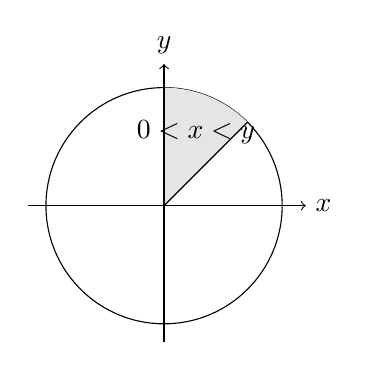
\begin{tikzpicture}[scale=1.5]
\draw (0,0) circle(1);\fill[gray!20] (0,0)--(45:1) arc[start angle=45,end angle=90,radius=1]--cycle;
\draw[->] (-1.15,0)--(1.2,0) node[right]{$x$};\draw[->] (0,-1.15)--(0,1.2) node[above]{$y$};\draw (0,0)--(45:1);\node at (.27,.62){$0<x<y$};
\end{tikzpicture}\end{center}
(c)\label{sol:flf19-7-c} 当 $0\leq z\leq1$, $Z\leq z$ 是半径 $\sqrt z$ 的圆盘, 面积比为 $z$. 因而 $F_Z(z)$ 在此区间为 $z$, 外侧为0或1, 密度 $f_Z(z)=1$ ($0<z<1$), 即 $Z\sim U[0,1]$.
\end{solution}

\begin{exercise}\label{ex:flf19-8}
原卷第8题. 垃圾邮件发送者Sally每天发大量邮件, 诱导收件人授权她完全访问银行账户. 授权时刻 $X_1,X_2,\ldots$ 以年为单位, 形成率 $\lambda=3$ 的Poisson点过程. (a) $Y=X_3$, 求 $f_Y$. (b) 首年获至少3次授权的概率? (c) $Y_0=0$, $Y_k=X_k-k/3$, 序列是否鞅? 解释.
\end{exercise}
\begin{solution}
(a)\label{sol:flf19-8-a} 三次到达时间是三段独立 $\Exp(3)$ 之和, Gamma密度为 $f_Y(y)=3^3y^2\ee^{-3y}/2!$, $y\geq0$.
(b)\label{sol:flf19-8-b} 首年计数为 $\Pois(3)$, 所求 $1-\ee^{-3}(1+3+9/2)=1-(17/2)\ee^{-3}$.
(c)\label{sol:flf19-8-c} 按到达序号而非连续日历时间取过滤 $\mathcal F_k=\sigma(X_1,\ldots,X_k)$. 间隔 $I_{k+1}=X_{k+1}-X_k$ 独立于过去且均值 $1/3$, 每个 $Y_k$ 可积并适应, 因此 $\E[Y_{k+1}\mid\mathcal F_k]=Y_k+1/3-1/3=Y_k$, 是鞅.
\end{solution}

\begin{exercise}\label{ex:flf19-9}
原卷第9题. 3人各有4顶不同帽, 全12帽放入箱中再均匀随机均分, 每人取4帽. $A_i$ 是第 $i$ 人全拿回自己的4帽事件, $N$ 为发生该事件的人数. (a) 求 $a=\Prob A_1$, $b=\Prob(A_1A_2)$. (b) 求 $\E N,\Var N$, 可用 $a,b$. (c) 求 $\Prob(N>0)$, 可用 $a,b$.
\end{exercise}
\begin{solution}
(a)\label{sol:flf19-9-a} 第一人所得是 $\binom{12}4=495$ 个四帽子集之一, 只有一个正确, 故 $a=1/495$. 给定第一人全对, 第二人从剩8帽中取4, 全对概率 $1/\binom84=1/70$. 故 $b=1/34650$.
(b)\label{sol:flf19-9-b} 令 $I_i=\ind_{A_i}$, $N=I_1+I_2+I_3$, 均值 $3a$. 平方有3个对角项、6个有序交叉项, 二阶矩 $3a+6b$, 因而方差 $3a+6b-9a^2$.
(c)\label{sol:flf19-9-c} 若前两人全对, 剩下4帽必是第三人的, 所以 $\Prob(A_1A_2A_3)=b$. 三对交集由对称性都为 $b$, 包含排除给 $\Prob(\cup_iA_i)=3a-3b+b=3a-2b$. 特别地, 恰有2人全对不可能.
\end{solution}

\begin{exercise}\label{ex:flf19-10}
原卷第10题. $X_i$ 独立同分布, 取0、1、2的概率分别 $1/8,3/4,1/8$, $S_n=\sum_{i=1}^nX_i$, $A_n=S_n/n$. (a) 求 $M_{S_{50}}(t)$ 与 $M_{A_{50}}(t)$. (b) 求单项均值、方差. (c) 用CLT近似 $\Prob(S_{100}>110)$, 可用 $\Phi$. (d) 求 $\rho(S_{50},S_{200})$.
\end{exercise}
\begin{solution}
(a)\label{sol:flf19-10-a} 单项矩母函数为 $m(t)=1/8+(3/4)\ee^t+(1/8)\ee^{2t}$. 独立性得 $M_{S_{50}}(t)=m(t)^{50}$, 缩放得 $M_{A_{50}}(t)=m(t/50)^{50}$.
(b)\label{sol:flf19-10-b} $\E X=3/4+2/8=1$, $\E X^2=3/4+4/8=5/4$, 方差 $1/4$.
(c)\label{sol:flf19-10-c} 总和均值100、方差25、标准差5, 门槛为2标准差, 原卷的CLT近似是 $1-\Phi(2)\approx.0228$. 因整数事件实际为 $S_{100}\geq111$, 若另采用半格连续性修正则门槛110.5, 得 $1-\Phi(2.1)$; 两者都是有限样本近似, 不是精确概率.
(d)\label{sol:flf19-10-d} $S_{200}=S_{50}+(S_{200}-S_{50})$, 后者独立于前者. 所以协方差 $\Var S_{50}=50/4$, 两方差为 $50/4,200/4$, 得相关 $(50/4)/\sqrt{(50/4)(200/4)}=1/2$.
\end{solution}

\originalsection{Practice Final练习卷}
本节对应\href{https://ocw.mit.edu/courses/18-600-probability-and-random-variables-fall-2019/resources/mit18_600f19_prc_final/}{官方练习卷}与\href{https://ocw.mit.edu/courses/18-600-probability-and-random-variables-fall-2019/resources/mit18_600f19_prc_final_soln/}{官方解答文件}. PDF印题名为``18.440 Practice Final Exam'', 分值合计100. 说明为: 本练习仅覆盖第二次期中以后内容, 实际期末覆盖全课程; 每题须清楚展示工作并框出结果. 官方文件对I、II、VI仅给教材/课件/作业阅读指引, 无本卷内实质解答. 这三题以下标为AI补写推导, 不冒充官方答案. 其余题依据官方解答重构, 补齐推导.

\begin{exercise}\label{ex:flp-I}
原卷I(20分). $X$ 有有限均值 $\mu$ 与方差 $\sigma^2$, $X_i$ 为独立同分布实例. CLT称 $T_n=(\sum_{i=1}^nX_i-n\mu)/(\sigma\sqrt n)$ 依分布趋于标准正态, 即对实数 $a$,
$\Prob(T_n<a)\to\int_{-\infty}^a\ee^{-x^2/2}\dd x/\sqrt{2\pi}$. 在矩母函数存在且定义良好的前提下, 按下列六步证明 $T_n$ 的矩母函数趋于标准正态矩母函数.
\begin{enumerate}
\item 解释为何只需考虑均值0、方差1的 $X$, 随后可假设如此.
\item $M_X(t)=\E\ee^{tX}$, 证明 $M_{T_n}(t)=M_X(t/\sqrt n)^n$, 且 $M_X'(0)=0$, $M_X''(0)=1$.
\item $L_X(t)=\ln M_X(t)$, 证明 $L_{T_n}(t)=nL_X(t/\sqrt n)$.
\item 证明 $L_X'(0)=0$, $L_X''(0)=\sigma^2=1$.
\item $N$ 标准正态, 证明 $L_N(t)=t^2/2$.
\item 用Taylor展开证明固定 $t$ 时 $L_{T_n}(t)\to L_N(t)$. 可用 $R(h)=R(0)+R'(0)h+R''(0)h^2/2+o(h^2)$ 的二阶展开.
\end{enumerate}
\end{exercise}
\begin{solution}
本题为AI补写推导. 先把原文``存在且定义良好''精确化: 要求 $\sigma>0$, 且存在 $\delta>0$ 使原变量的 $M_X(t)$ 在 $|t|<\delta$ 有限. 仅有限方差不保证矩母函数存在, 例如某些多项式尾分布; 下面是额外指数可积性下的MGF路线, 不是一般CLT的全部证明.

(1)\label{sol:flp-I-1} 令 $U_i=(X_i-\mu)/\sigma$, 它们独立同分布, 均值0方差1, 且原 $T_n=n^{-1/2}\sum U_i$. 因 $M_U(t)=\ee^{-t\mu/\sigma}M_X(t/\sigma)$, 标准化保留某个零点开邻域中的有限MGF. 若 $\sigma=0$, $X=\mu$ 几乎必然, 题中标准化无定义且不能得到非退化正态. 以下按题意将标准化变量重新记为 $X$.

(2)\label{sol:flp-I-2} 在相应存在范围内, 独立性给
\[M_{T_n}(t)=\E\prod_{i=1}^n\ee^{tX_i/\sqrt n}
=\prod_{i=1}^nM_X(t/\sqrt n)=M_X(t/\sqrt n)^n.\]
为保证求导可移入期望, 取 $0<\eta<\delta$. 两端 $M_X(\eta),M_X(-\eta)$ 有限, 因而 $\E\ee^{\eta|X|}<\infty$ (用 $\ee^{\eta|x|}\leq\ee^{\eta x}+\ee^{-\eta x}$). 对 $|t|\leq\eta/2$ 与 $k=1,2$, $|X|^k\ee^{tX}\leq C_{k,\eta}\ee^{\eta|X|}$, 因多项式能被剩余半指数控制. 控制收敛使 $M_X$ 至少二次连续可导, $M_X^{(k)}(t)=\E[X^k\ee^{tX}]$. 所以 $M_X'(0)=\E X=0$, $M_X''(0)=\E X^2=1$, 且 $M_X(0)=1$.

(3)\label{sol:flp-I-3} 实矩母函数严格正, 可取自然对数而不涉及分支. 由(2)得到 $L_{T_n}(t)=\ln M_X(t/\sqrt n)^n=nL_X(t/\sqrt n)$. 此处 $\ln$ 不是熵中的 $\log_2$.

(4)\label{sol:flp-I-4} 直接微分,
\[L_X'(t)=\frac{M_X'(t)}{M_X(t)},\qquad
L_X''(t)=\frac{M_X''(t)}{M_X(t)}-\left(\frac{M_X'(t)}{M_X(t)}\right)^2.\]
零点分别给0及 $\E X^2-(\E X)^2=1$. 由(2)中的二次连续可导和 $M_X>0$, $L_X$ 在零附近二次连续可导, 足以应用带 $o(h^2)$ 余项的Taylor展开.

(5)\label{sol:flp-I-5} 配方 $tx-x^2/2=-(x-t)^2/2+t^2/2$, 与题\ref{ex:fl17-5}的完整积分相同, 给 $M_N(t)=\ee^{t^2/2}$, 所以 $L_N(t)=t^2/2$.

(6)\label{sol:flp-I-6} (4)与 $L_X(0)=0$ 给 $L_X(h)=h^2/2+o(h^2)$. 固定 $t\ne0$, 令 $h=t/\sqrt n$, 则
\[L_{T_n}(t)=n\left(\frac{t^2}{2n}+o(1/n)\right)\longrightarrow\frac{t^2}{2}.
\]
$t=0$ 时两边恒零. 对每个固定实数 $t$, 足够大 $n$ 使 $t/\sqrt n$ 落入存在邻域, 这说明每个固定 $t$ 上最终有定义且MGF趋 $\ee^{t^2/2}$. 若还要由这一极限推出分布收敛, 需调用正文已声明的MGF连续性定理: 在零点一个共同开邻域内, MGF趋于某概率分布的有限MGF, 则对应分布趋于该分布. 这里可选择标准化后MGF原有的小邻域, 所有 $n$ 的MGF均存在于其中, 极限是标准正态MGF, 故工具的条件满足. 本题证明的是极限计算, 不将该分析工具的引用说成本题已证明了它. 也不从CLT的分布收敛反向推MGF收敛, 因后者通常需要额外尾部控制.
\end{solution}

\begin{exercise}\label{ex:flp-II}
原卷II(15分). 陈述强大数定律与弱大数定律, 并解释为什么强大数定律蕴含弱大数定律.
\end{exercise}
\begin{solution}\label{sol:flp-II}
本题为AI补写推导. 对独立同分布且 $\E|X_1|<\infty$ 的 $X_i$, 记 $\mu=\E X_1$, $A_n=n^{-1}\sum_{i=1}^nX_i$. 一般强大数定律声明 $\Prob(A_n\to\mu)=1$; 弱大数定律声明对每个 $\eps>0$, $\Prob(|A_n-\mu|>\eps)\to0$. 一般可积版强律在这里仅作为引用的定理陈述: 第9章完整本地证明的是 $\E|X_1|^4<\infty$ 版本, 而有限均值弱律已本地证明. 不把那份四阶矩证明宣称为一般可积版证明.

蕴含关系本身不需要独立性或矩条件, 只需已有几乎必然收敛. 固定 $\eps>0$, 令 $B_m=\bigcup_{n\geq m}\{|A_n-\mu|>\eps\}$. $B_m$ 递减, 交集是偏差超过 $\eps$ 无限次出现的事件, 在收敛的路径上不可能发生, 故其概率零. 概率从上连续性给 $\Prob(B_m)\to0$, 而 $\Prob(|A_m-\mu|>\eps)\leq\Prob(B_m)$, 得弱律. 这证明的只是强到弱的逻辑推论, 不承担强律存在性定理的证明.
\end{solution}

\begin{exercise}\label{ex:flp-III}
原卷III(10分). $X,Y$ 为独立公平三面骰点数, 各均匀取1、2、3, $Z=X+Y$. (1) 求 $H(X),H(Y),H(Z),H(X,Y)$. (2) 证明 $H(X,Y)=H(X,Z)$. (3) 显式计算两边验证 $H(X,Z)=H(Z)+H_Z(X)$.
\end{exercise}
\begin{solution}
本题依据官方解答重构, 补齐推导, 全部熵以比特计.
(1)\label{sol:flp-III-1} $H(X)=H(Y)=\log_2 3$, 联合九个等可能结果给 $H(X,Y)=\log_2 9=2\log_2 3$. $Z=2,3,4,5,6$ 的概率分别为 $1/9,2/9,3/9,2/9,1/9$, 因而
\begin{align*}
H(Z)&=-2\frac19\log_2\frac19-2\frac29\log_2\frac29-\frac39\log_2\frac39\\
&=\frac53\log_2 3-\frac49\log_2 2.
\end{align*}
(2)\label{sol:flp-III-2} 映射 $(x,y)\mapsto(x,x+y)$ 是一一对应, 逆映射 $(x,z)\mapsto(x,z-x)$. 所以 $(X,Z)$ 也有九个等可能结果, 熵 $2\log_2 3$, 与联合 $(X,Y)$ 相同.
(3)\label{sol:flp-III-3} 给定 $Z=2,3,4,5,6$, $X$ 分别在1、2、3、2、1个可能值中等可能, 条件熵分别为 $0,\log_2 2,\log_2 3,\log_2 2,0$. 按 $Z$ 加权得
$H_Z(X)=(4/9)\log_2 2+(1/3)\log_2 3$. 与(1)相加, $\log_2 2$ 项抵消, $\log_2 3$ 系数 $5/3+1/3=2$, 正好等于(2).
\end{solution}

\begin{exercise}\label{ex:flp-IV}
原卷IV(10分). Elaine旧车每天早晨有三态: 在她手中但坏了B、在她手中且可用W、在修理店S. 若早晨B, 次晨以 $.5$ 留B、$.5$ 去S; 若早晨S, 次晨以 $.75$ 留S、$.25$ 去W; 若早晨W, 次晨以 $.75$ 留W、$.25$ 去B. 长期有百分之几的早晨处于W?
\end{exercise}
\begin{solution}\label{sol:flp-IV}
依据官方解答重构, 补齐推导. 按B、W、S排序,
\[P=\begin{pmatrix}.5&0&.5\\.25&.75&0\\0&.25&.75\end{pmatrix}.\]
三态循环流平衡给 $\pi_B(.5)=\pi_W(.25)$, $\pi_W(.25)=\pi_S(.25)$, 所以 $\pi_W=\pi_S=2\pi_B$. 归一化给 $(\pi_B,\pi_W,\pi_S)=(.2,.4,.4)$. 链有限不可约, 时间比例等于唯一平稳分布, 所求40\%.
\end{solution}

\begin{exercise}\label{ex:flp-V}
原卷V(20分).
\begin{enumerate}
\item $X_1,X_2,\ldots$ 独立且期望为1. 以下哪些 $Y_n$ 必定是鞅?
\begin{enumerate}[label=(\alph*)]
\item $Y_n=X_n-1$.
\item $Y_n=X_n^2-1$.
\item $Y_n=7$.
\item $Y_n=n-\sum_{i=1}^nX_i$.
\item $Y_n=n-\sum_{i=1}^ni^2X_i$.
\item $Y_n=\prod_{i=1}^nX_i$.
\item $Y_n=\sum_{i=1}^nX_n^2-2n$. (保留原PDF中平方下标 $n$.)
\item $Y_n=\prod_{i=1}^nX_i^2$.
\end{enumerate}
\item 若 $Y_n$ 为鞅, 以下哪些必定是停时?
\begin{enumerate}[label=(\alph*)]
\item 首次 $Y_n>17$ 的时刻.
\item 最后一次 $Y_n=17$ 的时刻.
\item 首次 $Y_n=Y_{n+1}$ 的时刻.
\end{enumerate}
\item 举例说明鞅 $M_n$ 与停时 $T$ 可满足 $M_0=1$ 几乎必然, 但 $\E M_T=0$, 并解释不违背可选停止定理.
\end{enumerate}
\end{exercise}
\begin{solution}
依据官方解答重构, 补齐推导. 第一组相对于 $\mathcal F_n=\sigma(X_1,\ldots,X_n)$, ``期望1''按通常约定指有限期望, 因此 $X_i$ 可积. 未给二阶矩时不能额外假设平方可积. 题中必要成立的答案只有(1)(c)、(d)、(f).

(1)(a)\label{sol:flp-V-1-a} 不必定. 取独立 $X_n$ 各以 $1/2$ 取0、2. $Y_n$ 取 $-1,1$, 可积且适应, 但 $\E[Y_{n+1}\mid\mathcal F_n]=0\ne Y_n$.
(1)(b)\label{sol:flp-V-1-b} 不必定. 同一例中 $Y_n=X_n^2-1$ 取 $-1,3$, 下一项条件均值1, 不等于当前项. 而一般只给 $\E|X_n|<\infty$ 时连 $\E|X_n^2-1|<\infty$ 都不保证.
(1)(c)\label{sol:flp-V-1-c} 必定. 常数7对任何过滤适应可积, 条件期望仍7.
(1)(d)\label{sol:flp-V-1-d} 必定. $Y_0=0$, $Y_{n+1}-Y_n=1-X_{n+1}$ 可积且独立于 $\mathcal F_n$, 均值0; 固定时刻有限和可积, 故满足鞅三条件.
(1)(e)\label{sol:flp-V-1-e} 不必定. 条件增量均值为 $1-(n+1)^2$, 除最初一步外并非零. 取所有 $X_i\equiv1$ 已给确定但非常数的 $Y_n=n-\sum i^2$, 所以不是鞅.
(1)(f)\label{sol:flp-V-1-f} 必定. 空积 $Y_0=1$, 独立性保证 $\E|Y_n|=\prod_{i=1}^n\E|X_i|<\infty$. 且 $\E[Y_{n+1}\mid\mathcal F_n]=Y_n\E X_{n+1}=Y_n$.
(1)(g)\label{sol:flp-V-1-g} 不必定. 原式求和里的每项都是 $X_n^2$, 故 $Y_n=nX_n^2-2n$. 取 $X_i\equiv1$ 即 $Y_n=-n$, 不是鞅. 原PDF这一 $n$ 很可能是指标笔误, 但这里不暗改为 $i$; 即使另研究 $\sum X_i^2-2n$, 在仅均值1条件下也不能保证可积或零均值增量, 同一常数例仍否定.
(1)(h)\label{sol:flp-V-1-h} 不必定. 取0/2的二点例, $\E X_i^2=2$, 因而 $\E Y_n=2^n$, 均值不恒定已排除鞅. 这反例各矩有限, 不依赖可积性失败; 一般平方乘积还可能不可积.

(2)(a)\label{sol:flp-V-2-a} 必定是允许 $\infty$ 的停时. $T=\inf\{n:Y_n>17\}$ 有 $\{T\leq m\}=\bigcup_{n=0}^m\{Y_n>17\}\in\mathcal F_m$. 若从1起观察, 将并集从1起不改证明. 原官方YES附``假定几乎必然有限''; 按允许无击中时 $T=\infty$ 的标准定义不需该附加条件. 若只许有限停时, 则需另给必击中假设.
(2)(b)\label{sol:flp-V-2-b} 不必定, 因最后一次需要未来不再返回的信息. 一个有限反例是 $Y_0=17$, 第1步公平到16或18, 第2步再独立公平 $\pm1$. 若第2步为17, 第3步再公平走到16或18后永久保持; 若第2步不为17, 则从此保持. 这是有界鞅. 若第2步回17, 最后时刻为2; 否则第2步为15或19, 最后时刻为0. 两事件各概率 $1/2$, 所以 $\{T\leq0\}$ 在初始平凡信息下无法判定, 不为停时. 反例避免了``最后一次不存在''的歧义.
(2)(c)\label{sol:flp-V-2-c} 不必定. 取 $Y_0=0$, $Y_1=0$ 概率 $1/2$, $Y_1=\pm1$ 各 $1/4$, 此后保持 $Y_1$. 这是有界鞅. 首个相邻相等时刻为0若 $Y_1=0$, 否则为1; $\{T\leq0\}=\{Y_1=0\}$ 非初始可测. 若题从1起, 将此过程整体后移一时刻, 同样说明需要下一时刻的信息.

(3)\label{sol:flp-V-3} 取 $M_n=1+\sum_{i=1}^n\xi_i$, 独立 $\xi_i$ 公平取 $\pm1$, 过滤为增量历史, $T=\inf\{n:M_n=0\}$. $M_n$ 每固定时刻可积且有零条件均值增量, 为鞅; $T$ 是首击中停时. 为证 $T<\infty$ 几乎必然, 对整数 $K>1$ 先停止于0或 $K$, 有界停止给从1先0的概率 $1-1/K$. 这不超过最终击中0概率, 令 $K\to\infty$ 得1. 因而 $M_T=0$ 几乎必然, 期望0.

这不违背可选停止: $T$ 无确定界限, $M_{T\wedge n}$ 也不被某个固定可积变量统一控制. 实际上 $M_{T\wedge n}\geq0$, 各期望均1, 却几乎必然趋0, 因而不可能一致可积; 否则能交换极限与期望, 导致 $1=0$. 还可证 $\E T=\infty$: 若有限, 有界增量使 $|M_{T\wedge n}|\leq1+T$ 可积, 控制收敛又会矛盾. 所以带有限期望停时及有界增量的版本同样不适用.
\end{solution}

\begin{exercise}\label{ex:flp-VI}
原卷VI(15分). 计算Black--Scholes推导中的若干量. $X\sim\Normal(0,\sigma^2)$, 可以用 $\Phi(a)=\int_{-\infty}^a\ee^{-x^2/2}\dd x/\sqrt{2\pi}$.
\begin{enumerate}
\item 求 $\E\ee^X$.
\item 固定实数 $A$, 求 $\E[\ee^X\ind_{\{X>A\}}]$.
\item 求 $\E\ind_{\{X>A\}}$.
\item $G(a)=0$ 若 $a<K$, $G(a)=a-K$ 若 $a\geq K$, 求 $\E G(\ee^X)$.
\item 若 $X$ 改为均值 $-\sigma^2/2$, 方差 $\sigma^2$ 的正态, 上述答案怎样改变?
\item 附加题: 解释上述计算如何导出风险中性股价为对数正态时的欧洲看涨期权Black--Scholes公式.
\end{enumerate}
\end{exercise}
\begin{solution}
本题为AI补写推导. 先按非退化情形 $\sigma>0$ 计算; 退化情形及 $K\leq0$ 在最后说明, 避免未经题面授权暗中删除边界.

(1)\label{sol:flp-VI-1} $X=\sigma N$ 的矩母函数给 $\E\ee^X=\ee^{\sigma^2/2}$. 也可在密度指数中配方 $x-x^2/(2\sigma^2)=-(x-\sigma^2)^2/(2\sigma^2)+\sigma^2/2$, 积分后平移的正态密度质量为1.

(2)\label{sol:flp-VI-2} 同一配方把带权密度化成均值 $\sigma^2$ 的正态密度乘一个常数, 故
\begin{align*}
\E[\ee^X\ind_{\{X>A\}}]
&=\frac1{\sigma\sqrt{2\pi}}\int_A^\infty\ee^{x-x^2/(2\sigma^2)}\dd x\\
&=\ee^{\sigma^2/2}\int_{(A-\sigma^2)/\sigma}^\infty\frac{\ee^{-u^2/2}}{\sqrt{2\pi}}\dd u\\
&=\ee^{\sigma^2/2}\Phi\left(\frac{\sigma^2-A}{\sigma}\right).
\end{align*}
最后使用 $1-\Phi(z)=\Phi(-z)$, 来源于标准正态对称性. 这种指数加权使均值移动 $\sigma^2$, 解释后面的两个不同 $d$ 参数.

(3)\label{sol:flp-VI-3} 指示变量期望等于事件概率, 标准化得 $\Prob(X>A)=1-\Phi(A/\sigma)=\Phi(-A/\sigma)$.

(4)\label{sol:flp-VI-4} 若 $K>0$, 因 $\ee^X>K$ 等价于 $X>\ln K$, 收益写成 $\ee^X\ind_{\{X>\ln K\}}-K\ind_{\{X>\ln K\}}$. 将(2)(3)取 $A=\ln K$, 得
\[\E G(\ee^X)=\ee^{\sigma^2/2}\Phi\left(\frac{\sigma^2-\ln K}{\sigma}\right)
-K\Phi\left(\frac{-\ln K}{\sigma}\right).\]
等号处收益0且正态无原子, 不影响严格/非严格阈值. 这里使用自然对数 $\ln$, 与熵对数不同.

(5)\label{sol:flp-VI-5} 为避免混淆, 暂记任意均值 $m$ 的变量为 $X=m+\sigma N$. 对(2)相同配方给通式
\[\E[\ee^X\ind_{\{X>A\}}]=\ee^{m+\sigma^2/2}\Phi\left(\frac{m+\sigma^2-A}{\sigma}\right),\qquad
\Prob(X>A)=\Phi\left(\frac{m-A}{\sigma}\right).\]
这是对 $m+\sigma N$ 代入前面零均值公式: 指数多出 $\ee^m$, 阈值减 $m$. 现在取 $m=-\sigma^2/2$, 得四个答案分别为
\begin{align*}
\E\ee^X&=1,\\
\E[\ee^X\ind_{\{X>A\}}]&=\Phi\left(\frac{\sigma^2/2-A}{\sigma}\right),\\
\E\ind_{\{X>A\}}&=\Phi\left(\frac{-\sigma^2/2-A}{\sigma}\right),\\
\E G(\ee^X)&=\Phi\left(\frac{\sigma^2/2-\ln K}{\sigma}\right)
-K\Phi\left(\frac{-\sigma^2/2-\ln K}{\sigma}\right)\quad(K>0).
\end{align*}
均值减去半方差正是令指数变量均值回到1的补偿, 而不令正态变量本身均值为0.

(6)\label{sol:flp-VI-6} 为讲清模型与工具调用, 假设无分红、当前股票价 $S_0>0$, 距到期 $\tau>0$, 无风险连续利率 $r$, 单位时间波动率 $v>0$. 假定已建立风险中性定价规则: 可复制欧洲看涨收益 $(S_T-K)^+$ 的当前价值为 $\ee^{-r\tau}\E_Q[(S_T-K)^+]$. 这规则来自正文的无套利/复制模型; 本题只计算给定规则下的期望, 不以积分本身证明市场存在完备风险中性模型.

在该模型风险中性分布为
\[S_T=S_0\exp\left((r-v^2/2)\tau+v\sqrt\tau N\right)
=S_0\ee^{r\tau}\ee^Z,\quad
Z\sim\Normal(-s^2/2,s^2),\quad s=v\sqrt\tau.\]
因此 $\E_Q S_T=S_0\ee^{r\tau}$, 贴现均值正好为 $S_0$. 对 $K>0$, 收益正的条件是 $Z>A$, $A=\ln(K/S_0)-r\tau$. 按(5),
\begin{align*}
C_0&=\ee^{-r\tau}\left(S_0\ee^{r\tau}\E_Q[\ee^Z\ind_{\{Z>A\}}]
-K\Prob_Q(Z>A)\right)\\
&=S_0\Phi(d_1)-K\ee^{-r\tau}\Phi(d_2),\\
d_1&=\frac{\ln(S_0/K)+(r+v^2/2)\tau}{v\sqrt\tau},\qquad
 d_2=\frac{\ln(S_0/K)+(r-v^2/2)\tau}{v\sqrt\tau}=d_1-v\sqrt\tau.
\end{align*}
两项分别来自股价加权尾概率与普通尾概率, 因而必须使用两个不同的 $d$. 取 $r=0,S_0=1$ 就回到(5)的看涨公式. 若有连续分红率 $q$, 在已声明相应风险中性模型的前提下将 $r$ 换为 $r-q$ 并将第一项乘 $\ee^{-q\tau}$, 但原题未要求这一推广.

边界核查: 若 $K\leq0$, $\ee^X$ 总为正, 收益恒 $\ee^X-K$, 所以(4)为 $\ee^{\sigma^2/2}-K$, (5)为 $1-K$, 无需 $\ln K$. 若 $\sigma=0$, 两种给定均值都是0, 所以 $X=0$ 几乎必然: (1)为1, (2)(3)均为 $\ind_{\{0>A\}}$, (4)(5)为 $(1-K)^+$. 附加题中若 $v=0$ 或 $\tau=0$, 可直接用确定股价的贴现收益, 不能在 $d_1,d_2$ 中除以零.
\end{solution}

\begin{exercise}\label{ex:flp-VII}
原卷VII(10分). 利息与分红都为零, 某股票到期日 $T$ 的欧洲看涨期权, 行权价 $K\geq0$ 对应当前价 $C(K)=\ee^{-K}$. (1) 股票现在价值必须是多少? (2) 风险中性下到期股票价在 $[5,10]$ 的概率? (3) 若到期股票价为 $X$, 支付 $X^2$ 的合约现在价值多少?
\end{exercise}
\begin{solution}
依据官方解答重构, 补齐推导. 股票到期价 $X\geq0$, 风险中性定价为 $C(K)=\E[(X-K)^+]$. 为从call函数恢复分布, 对固定 $x$ 的折线 $(x-K)^+$ 取右导, 得 $-\ind_{\{x>K\}}$. 差商绝对值不超过1, 可交换极限与期望, 所以 $C'_+(K)=-\Prob(X>K)=F_X(K)-1$. 给定函数光滑, 得 $F_X(K)=1-\ee^{-K}$ ($K\geq0$), 包括 $F_X(0)=0$; 再求导得到风险中性密度 $f_X(x)=\ee^{-x}$ ($x>0$), 为 $\Exp(1)$.

(1)\label{sol:flp-VII-1} 利息为零时股票当前价为风险中性均值 $\E X=1$. 也可直接由 $C(0)=\E X=1$ 得到, 因0行权价看涨恰支付非负股价.
(2)\label{sol:flp-VII-2} 密度连续无原子, 区间端点无影响, 概率 $F_X(10)-F_X(5)=\ee^{-5}-\ee^{-10}$.
(3)\label{sol:flp-VII-3} 零利率下支付 $X^2$ 的价格为 $\E X^2=\int_0^\infty x^2\ee^{-x}\dd x=2!=2$. 这依赖题目规定的风险中性定价模型; 风险中性概率不是实际世界的统计频率.
\end{solution}
